\clearpage
\Question{Graph Traversals}

\begin{parts}

\part[1]\TAGS{graph, traverse-ds}
Consider the following 11-vertex graph:
\begin{center}\vspace{-2ex}%
\hspace*{15em}
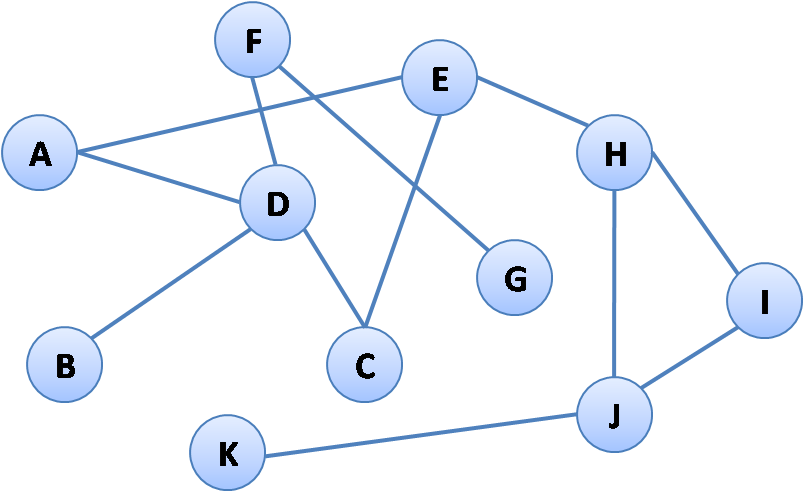
\includegraphics[width=.5\textwidth]{\img/dfsbfsgraph.png}
\end{center}

Using recursive depth-first traversal, list the vertices in the order they
are visited as we search from vertex $A$ to vertex $J$.  When we visit
a vertex, we explore its outgoing edges in alphabetical order.

\begin{framed}
\medskip
\answer{34em}{A, \ D, \ B, \ C, \ E, \ H, \ I, \ (J)}\phantom{|}
\end{framed}

Using breadth-first traversal, list the vertices in the order that
they are visited as we search from vertex $A$ to vertex $J$. When we
visit a node, we explore its outgoing edges in alphabetical order.

\begin{framed}
\medskip
\answer{34em}{A, \ D, \ E, \ B, \ C, \ F, \ (H, \ I, \ J)}\phantom{|}
\end{framed}

\RUBRIC
Part (a)
TAGS: graph, traverse-ds

Gradescope rubric:
+0.25pt: (DFS) first 3 nodes are A, D, B
+0.25pt: (DFS) remaining nodes are C, E, H, I (J optional)
+0.25pt: (BFS) first 3 nodes are A, D, E
+0.25pt: (BFS) remaining nodes are B, C, F, H, (G, I, J optional)

Commentary:
  Accept shortcut answer where search stops when target is about to be
  put in stack/queue

  DFS:
  A, D, B, C, E, H, I, J <- Last 1 optional
  ^^^^^^^
  1/2pt if they at least get this part
  Need to leave off K and G for full credit

  Marked        <>Stack (top to the left)
  A             A
  A  DE         D, E
  ABCDEF        B, C, F, E
  ABCDEF        C, F, E
  ABCDEFG       G, F, E
  ABCDEFG       F, E
  ABCDEFG       E
  ABCDEFG I     I
  ABCDEFG IJK   J, K

  BFS:
  A, D, E, B, C, F, H, I, J <-- Last 3 optional
  ^^^^^^^
  1/4 point if they at least get this point

  Marked        <Queue<
  A             A
  A  DE         D, E
  ABCDEF        E, B, C, F
  ABCDEF H      B, C, F, H
  ABCDEF H      C, F, H
  ABCDEFGH      F, H, G
  ABCDEFGHIJ    H, I, J        <-- ACCEPT
  ABCDEFGKIJ    I, J
  ABCDEFGKIJ    J
ENDRUBRIC


\part[1]\TAGS{graph}
For an undirected graph with $n$ vertices, what is the maximum number
of edges this graph can have? (This is called a \emph{complete
  graph}). Express your answer in closed form as a function of $n$.
\begin{framed}
\medskip
\answer{34em}{$n(n-1)/2$}\phantom{|}
\end{framed}

A politician must plan a trip to visit $n$ cities and give a speech
once at each city and then return home, starting and ending in the
politician's home city (which is one of the $n$ cities). The
politician can fly directly from any city to any other city. The
politician does not want to visit each city more than once and wants
to return back to the home city at the end of the trip. The
politician's staff wants to figure out all of the possible trips that
the politician can make to determine which will have the maximum
impact on voters.

Express the number of possible unique trips to visit the $n$ cities in
big-O notation as a function of $n$ in its simplest, tightest
form. (HINT: Think about this as a complete graph.)
\begin{framed}
\medskip
$O(\uanswer{16em}{$n!$})$
\end{framed}

\RUBRIC
Part (b)
TAGS: graph

Gradescope rubric:
+0.5pt  (1st blank): -- EITHER  n(n-1)/2 = (n^2-n)/2 = n choose 2
+0.25pt (1st blank): -- OR O(n^2)
+0.5pt  (2nd blank): -- EITHER  O((n-1)!)
+0.25pt (2nd blank): -- OR O(n!)

Commentary:
  Half points: n(n-1)/2 = (n^2-n)/2 = n choose 2
  Half of that for O(n^2) or anything in there

  Half points: O((n-1)!)
  Half of that: O(n!)
ENDRUBRIC

\end{parts}
